\contourlength{1.0pt}
\tikzset{>=latex} % for LaTeX arrow head

\colorlet{xcol}{blue!60!black}
\colorlet{myred}{red!80!black}
\colorlet{myblue}{blue!80!black}
\colorlet{mygreen}{green!40!black}
\colorlet{myorange}{orange!90!black}
\colorlet{mypurple}{red!50!blue!90!black!80}
\colorlet{mydarkred}{myred!80!black}
\colorlet{mydarkblue}{myblue!80!black}
\tikzstyle{xline}=[xcol,thick]
\tikzstyle{width}=[{Latex[length=5,width=3]}-{Latex[length=5,width=3]},thick]
\tikzset{
  traj/.style 2 args={xline,postaction={decorate},decoration={markings,
    mark=at position #1 with {\arrow{<}},
    mark=at position #2 with {\arrow{<}}}
  }
}
\def\tick#1#2{\draw[thick] (#1)++(#2:0.12) --++ (#2-180:0.24)}
\def\N{100} % number of samples

% CIRCLE on axis




% RESONANCE


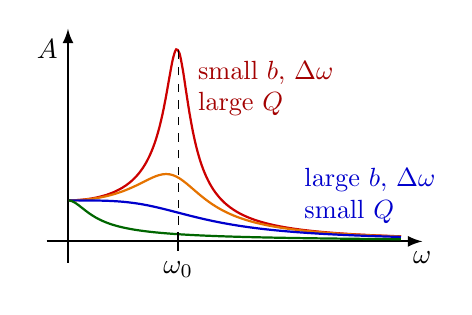
\begin{tikzpicture}
  \def\xmax{4.5}
  \def\ymax{2.7}
  \def\c{1.4}        % natural frequency
  \def\A{0.90*\ymax} % amplitude
  \def\ba{0.3}       % drag coefficient 1
  \def\bb{0.9}       % drag coefficient 2
  \def\bc{2.0}       % drag coefficient 3
  \def\bd{8.0}       % drag coefficient 4
  \coordinate (O) at (0,0);
  \coordinate (X) at (\xmax,0);
  \coordinate (Y) at (0,\ymax);
  \coordinate (C) at (\c,0);
  
  % AXIS
  \draw[->,thick]
    (-0.1*\ymax,0) -- (\xmax,0) node[below] {$\omega$};
  \draw[->,thick]
    (0,-0.1*\ymax) -- (0,\ymax) node[below left] {$A$}; %\langle{P}\rangle
  
  % PLOT
  \draw[xline,myred,samples=\N,smooth,variable=\x,domain=0.01:0.94*\xmax]
    plot(\x,{\A*\ba*\c/sqrt((\c*\c-\x*\x)^2 + (\ba*\x)^2 )});
  \draw[xline,myorange,samples=\N,smooth,variable=\x,domain=0.01:0.94*\xmax]
    plot(\x,{\A*\ba*\c/sqrt((\c*\c-\x*\x)^2 + (\bb*\x)^2 )});
  \draw[xline,myblue,samples=\N,smooth,variable=\x,domain=0.01:0.94*\xmax]
    plot(\x,{\A*\ba*\c/sqrt((\c*\c-\x*\x)^2 + (\bc*\x)^2 )});
  \draw[xline,mygreen,samples=\N,smooth,variable=\x,domain=0.01:0.94*\xmax]
    plot(\x,{\A*\ba*\c/sqrt((\c*\c-\x*\x)^2 + (\bd*\x)^2 )});
  \node[mydarkred,align=left,right,scale=0.95] at ({0.26*(\c+\xmax)},0.8*\A) {small $b$, $\Delta\omega$\\large $Q$};
  \node[myblue,align=left,above,scale=0.95] at ({0.65*(\c+\xmax)},0.3*\A*\ba/\bc) {large $b$, $\Delta\omega$\\small $Q$};
  \draw[dashed,thin] (C) --++ (0,\A);
  \tick{C}{90} node[below] {$\omega_0$};
  
  % WIDTH
  %\draw[<->,thick] ({\c/(2*\Q)*(-1+sqrt(1+4*\Q^2))},\A/2) -- ({\c/(2*\Q)*(1+sqrt(1+4*\Q^2))},\A/2);
  %\draw[width,myblue!80!black]
  %  ({\c/(2*\q)*(-1+sqrt(1+4*\q^2))},\a/2) --++ (\c/\q,0) node[midway,above] {$\Delta \omega$};
  %\draw[width,mydarkred]
  %  ({\c/sqrt(2*\Q)*(-1+sqrt(1+4*\Q^2))},\A/2) --++ {(\c/sqrt(\Q)},0)
  %  node[midway,left=0.8,above,scale=0.9] {\contour{white}{$\Delta \omega$}};
  
\end{tikzpicture}
